\begin{enumerate}[label=\thechapter.\arabic*,ref=\thechapter.\theenumi]

\item Consider the discrete time signal $x\sbrak{n} = u\sbrak{-n+5} - u\sbrak{n+3}$, where
\[u\sbrak{n} = 
\begin{cases}
    1;n\geq0\\
    0;n<0
\end{cases}
\]
The smallest n for which $x\sbrak{n} = 0$ is?
\hfill(GATE IN 2023)
\\ \solution
\input{2023/IN/28/gate1.tex}
\newpage
\item Two sequences $x_1\sbrak{n} $ and $ x_2 \sbrak{n}$ are described as follows:
\begin{align}
x_1\sbrak{0} = x_2\sbrak{0} = 1\\
x_1\sbrak{1} = x_2\sbrak{2} = 2\\
x_1\sbrak{2} = x_2\sbrak{1} = 1
\end{align}
$x_1\sbrak{n} = x_2\sbrak{n} = 0$ for all $n<0$ and $n>2$\\
\\
If $x\sbrak{n}$ is obtained by convoluting $x_1\sbrak{n}$ with $x_2\sbrak{n}$, which of the following equations is/are TRUE?\\
\\
(A) $x\sbrak{2} = x\sbrak{3}$\\
\\
(B) $x\sbrak{1} = 2$\\
\\
(C) $x\sbrak{4} = 3$\\
\\
(D) $x\sbrak{2} = 5$\\
\hfill(GATE 2023 BM 47)
\solution
\input {2023/BM/47/Gate2023_Bm_47.tex}
\pagebreak
\item A series \brak{S} is given as S=1+3+5+7+9+..... The sum of the first 50 terms of S is \underline{\hspace{1in}}
\hfill(GATE 2023 BT 32)
\\ \solution
\iffalse
\let\negmedspace\undefined
\let\negthickspace\undefined
\documentclass[journal,12pt,twocolumn]{IEEEtran}
\usepackage{cite}
\usepackage{amsmath,amssymb,amsfonts,amsthm}
\usepackage{algorithmic}
\usepackage{graphicx}
\usepackage{textcomp}
\usepackage{xcolor}
\usepackage{txfonts}
\usepackage{listings}
\usepackage{enumitem}
\usepackage{mathtools}
\usepackage{gensymb}
\usepackage{comment}
\usepackage[breaklinks=true]{adjustbox}
\usepackage{tkz-euclide} 
\usepackage{listings}
\usepackage{gvv}                                        
\def\inputGnumericTable{}                                 
\usepackage[latin1]{inputenc}                                
\usepackage{color}                                            
\usepackage{array}                                            
\usepackage{longtable}                                       
\usepackage{calc}                                             
\usepackage{multirow}                                         
\usepackage{hhline}                                           
\usepackage{ifthen}                                           
\usepackage{lscape}

\newtheorem{theorem}{Theorem}[section]
\newtheorem{problem}{Problem}
\newtheorem{proposition}{Proposition}[section]
\newtheorem{lemma}{Lemma}[section]
\newtheorem{corollary}[theorem]{Corollary}
\newtheorem{example}{Example}[section]
\newtheorem{definition}[problem]{Definition}
\newcommand{\BEQA}{\begin{eqnarray}}
\newcommand{\EEQA}{\end{eqnarray}}
\newcommand{\define}{\stackrel{\triangle}{=}}
\theoremstyle{remark}
\newtheorem{rem}{Remark}

\begin{document}
\bibliographystyle{IEEEtran}

\vspace{3cm}

\title{}
\author{EE23BTECH11024 - G.Karthik Yadav$^{*}$
}
\maketitle
\newpage
\bigskip

\section*{GATE 2023 EC 41}
\noindent 1. \hspace{2pt} A Closed loop systen is shown in the figure where $k>0$ and $\alpha>0$ .\\
The Steady State error due to a ramp input $\brak{R\brak{s} = \alpha s^{-2}}$ is given by \hfill{(GATE 2023 EC 41)}

\begin{figure}[ht]
\centering
    \includegraphics[width=1.0\linewidth]{2023/EC/41/figs/question.png}
    \label{fig: 23.EC.41.24.1}
\end{figure}

\begin{enumerate}
\item $\frac{2\alpha}{k}$
\item $\frac{\alpha}{k}$
\item $\frac{\alpha}{2k}$
\item $\frac{\alpha}{4k}$
\end{enumerate}

\solution\\
\fi
\begin{table}[ht]
\setlength{\arrayrulewidth}{0.3mm}
\setlength{\tabcolsep}{15pt}
\renewcommand{\arraystretch}{1.5}



\begin{tabular}{ |p{1cm}|p{3cm}|p{1cm}| }
\hline
Symbol & Parameters & Value\\
\hline
$R\brak{s}$ & Laplace transform Ramp input signal r\brak{t} &  $\alpha s^{-2}$\\
\hline
$G\brak{s}$ & Open Loop transfer function &  $ \frac{Y\brak{s}}{E\brak{s}} = \frac{k}{s\brak{s+2}}$\\
\hline
$Y\brak{s}$ & Laplace transform of the output signal y\brak{t}  &  ? \\
\hline
$E\brak{s}$ & Laplace transform of the error signal e\brak{t} & R\brak{s} - Y\brak{s}\\
\hline
$E\brak{s}$ & Laplace transform of the error signal e\brak{t} & R\brak{s} - Y\brak{s}\\   
\hline
$e_s$ & Steady State Error &  ? \\
\hline
%$x(l)$ & Last($l^{th}$) term of series & 350\\
%$x(0)$ & Starting ($0^{th}$) term of series & 17 %\\
%\hline
%d & Common difference of AP & 9\\
%\hline
\end{tabular}
\caption{Parameters}






\end{table}
\bigskip
from table  Open loop transfer function $G\brak{s}$\\
\begin{align}
	G\brak{s} &= \frac{Y\brak{s}}{E\brak{s}} \label{24.2023.EC.41.1} \\
        &= \frac{Y\brak{s}}{R\brak{s} - Y\brak{s}} \\
        Y\brak{s} &= \frac{R\brak{s}G\brak{s}}{1 + G\brak{s}} \label{24.2023.EC.41.2}
\end{align}

from eq \ref{24.2023.EC.41.1} and eq \eqref{24.2023.EC.41.2}

\begin{align}
        G\brak{s} &= \frac{k}{s\brak{s +2}}  \label{24.2023.EC.41.3} \\ 
        Y\brak{s} &= \frac{\alpha k s^{-2}}{k + s\brak{s+2}} \label{24.2023.EC.41.4} \\
        E\brak{s} &= R\brak{s} - Y\brak{s}  \label{24.2023.EC.41.5} \\ 
        E\brak{s} &= \frac{\alpha \brak{s+2}}{s\brak{k + s\brak{s+2}}}
\end{align}

By Taking Inverse Laplace Transform of eq \eqref{24.2023.EC.41.3} and eq\eqref{24.2023.EC.41.4}

\begin{align}
    g\brak{t} &= \frac{k\brak{1 - e^{-2t}}}{2} u\brak{t} \\
        y\brak{t} &= \alpha t u\brak{t}- \frac{2\alpha}{k}u\brak{t} \\
        \notag &+\frac{\alpha}{2k\sqrt{1-k}} \biggl(2\sqrt{1-k}e^{\sqrt{1-k}t-1}\\ 
        \notag &+ 2\sqrt{1-k}e^{-\sqrt{1-k}t-1} \\
        \notag &+ \brak{2-k}e^{\sqrt{1-k}t-1} - \brak{2-k}e^{-\sqrt{1-k}t-1} \biggr) u\brak{t}
\end{align}

\begin{align}
        e\brak{t} &= r\brak{t} - y\brak{t} \\
        &= \alpha t u\brak{t} - y\brak{t} \\
        e\brak{t} &= \frac{2\alpha}{k}u\brak{t} \\
        \notag &-\frac{\alpha}{2k\sqrt{1-k}} \biggl(2\sqrt{1-k}e^{\sqrt{1-k}t-1}\\ 
        \notag &+ 2\sqrt{1-k}e^{-\sqrt{1-k}t-1} \\
        \notag &+ \brak{2-k}e^{\sqrt{1-k}t-1} - \brak{2-k}e^{-\sqrt{1-k}t-1} \biggr) u\brak{t}
\end{align}
	

\begin{align}
    e_s &= \displaystyle\lim_{s\to 0}s E\brak{s} \\
    &= \displaystyle\lim_{s\to 0} s \frac{R\brak{s}}{1 + G\brak{s}} \\
    &= \displaystyle\lim_{s\to 0} \frac{\alpha \brak{s+2}}{s\brak{s+2} + k} \\
    e_s &= \frac{2\alpha}{k}
\end{align}



\pagebreak

\item For the signals x\brak{t} and y\brak{t} shown in the figure, $z\brak{t}=x\brak{t}*y\brak{t}$ is maximum at $t=T_1$. Then $T_1$ in seconds is .......... \brak{\text{Round off to the nearest integer}}
\solution
\pagebreak

\item A series of natural numbers F$_1$, F$_2$, F$_3$, F$_4$, F$_5$, F$_6$, F$_7$,....obeys F$_{n+1}$ = F$_n$ + F$_{n-1}$ for all integers n $\geq$ 2. If F$_6$ = 37, and F$_7$ = 60, then what is F$_1$?\\  
 \hfill[GATE CS 2023] \\
 \solution 
 \input{2023/CS/3/SS-GATE.tex}
 \pagebreak

 \item The Lucas sequence $L_{n}$is defined by the recurrence relation:\\
\begin{align*}
    L_{n}=L_{n-1}+L_{n-2}, for n\geq3
\end{align*}
with $L_{1}$=1 and $L_{2}$=3\\
Which one of the option given is TRUE?\\
\begin{enumerate}
    \item $L_{n}=\brak{\frac{1+\sqrt{5}}{2}}^n+\brak{\frac{1-\sqrt{5}}{2}}^n$
    \item $L_{n}=\brak{\frac{1+\sqrt{5}}{2}}^n-\brak{\frac{1-\sqrt{5}}{3}}^n$
    \item $L_{n}=\brak{\frac{1+\sqrt{5}}{2}}^n+\brak{\frac{1-\sqrt{5}}{3}}^n$
    \item $L_{n}=\brak{\frac{1+\sqrt{5}}{2}}^n-\brak{\frac{1-\sqrt{5}}{2}}^n$
\end{enumerate}
\hfill{(GATE 2023 CS 15)}\\
\solution
\iffalse
\let\negmedspace\undefined
\let\negthickspace\undefined
\documentclass[journal,12pt,twocolumn]{IEEEtran}
\usepackage{cite}
\usepackage{amsmath,amssymb,amsfonts,amsthm}
\usepackage{algorithmic}
\usepackage{graphicx}
\usepackage{textcomp}
\usepackage{xcolor}
\usepackage{txfonts}
\usepackage{listings}
\usepackage{enumitem}
\usepackage{mathtools}
\usepackage{gensymb}
\usepackage{comment}
\usepackage[breaklinks=true]{hyperref}
\usepackage{tkz-euclide} 
\usepackage{listings}
\usepackage{gvv}                                        
\def\inputGnumericTable{}                                 
\usepackage[latin1]{inputenc}                                
\usepackage{color}                                            
\usepackage{array}                                            
\usepackage{longtable}                                       
\usepackage{calc}                                             
\usepackage{multirow}                                         
\usepackage{hhline}                                           
\usepackage{ifthen}                                           
\usepackage{lscape}
\newtheorem{theorem}{Theorem}[section]
\newtheorem{problem}{Problem}
\newtheorem{proposition}{Proposition}[section]
\newtheorem{lemma}{Lemma}[section]
\newtheorem{corollary}[theorem]{Corollary}
\newtheorem{example}{Example}[section]
\newtheorem{definition}[problem]{Definition}
\newcommand{\BEQA}{\begin{eqnarray}}
\newcommand{\EEQA}{\end{eqnarray}}
\newcommand{\define}{\stackrel{\triangle}{=}}
\theoremstyle{remark}
\newtheorem{rem}{Remark}
\begin{document}
\parindent 0px
\bibliographystyle{IEEEtran}
\title{Assignment CS\_15Q}
\author{EE23BTECH11028 - Kamale Goutham$^{}$% <-this % stops a space
}
\maketitle
\newpage
\bigskip
\section*{Question}
The Lucas sequence $L_{n}$is defined by the recurrence relation:\\
\begin{align*}
    L_{n}=L_{n-1}+L_{n-2}, for n\geq3
\end{align*}
with $L_{1}$=1 and $L_{2}$=3\\
Which one of the option given is TRUE?\\
\begin{enumerate}
    \item $L_{n}=\brak{\frac{1+\sqrt{5}}{2}}^n+\brak{\frac{1-\sqrt{5}}{2}}^n$
    \item $L_{n}=\brak{\frac{1+\sqrt{5}}{2}}^n-\brak{\frac{1-\sqrt{5}}{3}}^n$
    \item $L_{n}=\brak{\frac{1+\sqrt{5}}{2}}^n+\brak{\frac{1-\sqrt{5}}{3}}^n$
    \item $L_{n}=\brak{\frac{1+\sqrt{5}}{2}}^n-\brak{\frac{1-\sqrt{5}}{2}}^n$
\end{enumerate}
\hfill{(GATE 2023 CS 15)}\\
\solution\\
\fi
Initial condition $L_{1}$=1 and $L_{2}$=3
\begin{align}
 L_{n}=L_{n-1}+L_{n-2}
\end{align}
Assume $L_{n+1}=x(n)$\\
\begin{align}
 x(n)=&[x(n-1)+x(n-2)-3]u(n-2)+u(n)+2u(n-1)\\
 X(z)=&z^{-1}(X(z)-1)+z^{-2}X(z)-3\frac{z^{-2}}{1-z^{-1}}+\frac{1}{1-z^{-1}}+2\frac{z^{-1}}{1-z^{-1}}\\
 X(z)&(1-z^{-1}-z^{-2})(1-z^{-1})=1+z^{-1}-2z^{-2}\\
 X(z)&=\frac{1+z^{-1}-2z^{-2}}{(1-z^{-1}-z^{-2})(1-z^{-1})}\\
 X(z)&=\frac{A}{1-z^{-1}}+\frac{B}{1-\alpha z^{-1}}+\frac{C}{1-\beta z^{-1}}
 \end{align}
 Where, $\alpha$ = $\dfrac{1 +\sqrt{5}}{2}$ and $\beta$ = $\dfrac{1 -\sqrt{5}}{2}$ \\
 
	\vspace{0.4cm}
 using partial fractions,
 \begin{align}
     X(z)=\frac{\alpha+2}{(\alpha-\beta)(1-\alpha z^{-1})}+\frac{\beta+2}{(\beta-\alpha)(1-\beta z^{-1})}
 \end{align}
 
	$a^n u(n)$
	$\xleftarrow[]{\hspace{0.4cm}{\mathcal{Z}}\hspace{0.1cm}}\xrightarrow[]{}$
	$\dfrac{1}{1 - a z^{-1}}$ \hspace{0.2cm} $\lvert \hspace{0.1cm} z \hspace{0.1cm}\rvert \hspace{0.1cm} \textgreater \hspace{0.1cm} \lvert \hspace{0.1cm} a \hspace{0.1cm} \rvert$
	
	\vspace{0.4cm}
	
	Substituting this result,
	
	\vspace{-0.5cm}
	
	\begin{align}
		x(n) &= \dfrac{\alpha+2}{(\alpha - \beta)} (\alpha^n u(n)) - \dfrac{\beta+2}{(\alpha - \beta)} (\beta^n u(n))\\
	    x(n) &= \dfrac{(5+\sqrt{5})(1 + \sqrt{5})^{n} - (5-\sqrt{5})(1 - \sqrt{5})^{n} }{2^{n+1} \sqrt{5}} u(n)\\
    	x(n) &= \dfrac{(1 + \sqrt{5})^{n+1} +(1 - \sqrt{5})^{n+1} }{2^{n+1}} u(n)
    \end{align}
$\therefore$ $L_{n} =\brak{\frac{1+\sqrt{5}}{2}}^n+\brak{\frac{1-\sqrt{5}}{2}}^n$
option 1 is correct.
\newpage
\begin{figure}[h]
  \centering
  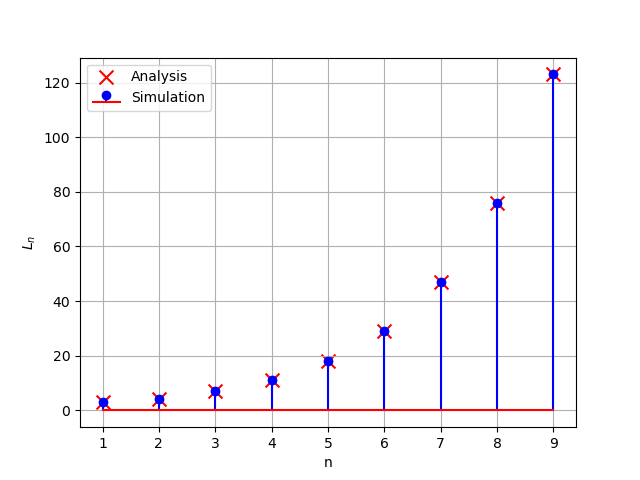
\includegraphics[width=\columnwidth]{2023/CS/15/figs/fig1.png}
  \caption{$L_{n}=\brak{\frac{1+\sqrt{5}}{2}}^n+\brak{\frac{1-\sqrt{5}}{2}}^n$}
\end{figure}

\pagebreak
\end{enumerate}
